\documentclass[titlepage]{scrartcl}
\usepackage{selinput}
\SelectInputMappings{
	adieresis={ä},
	germandbls={ß}
	}
\usepackage[T1]{fontenc}
\usepackage{lmodern}
\usepackage[ngerman]{babel}

\usepackage{eurosym}

\usepackage{graphicx}
\usepackage{booktabs}

\subject{Vortrag}
\title{Beispiel Dokument}
\subtitle{Mit Untertitel}
\author{Thomas Helmke}
\date{2014-05-06}
\publishers{Hackerspace Bremen e.V.}

\begin{document}
\maketitle

\tableofcontents
\listoffigures
\listoftables
\clearpage

\section{Erster Abschnitt}\label{sec:Kapitel1}
\subsection{Ein Unterabschnitt}
Dies ist ein Typoblindtext. An ihm kann man sehen, ob alle Buchstaben da sind und wie sie aussehen. Manchmal benutzt man Worte wie Hamburgefonts, Rafgenduks oder Handgloves, um Schriften zu testen. Manchmal Sätze, die alle Buchstaben des Alphabets enthalten - man nennt diese Sätze »Pangrams«. Sehr bekannt ist dieser: The quick brown fox jumps over the lazy old dog. Oft werden in Typoblindtexte auch fremdsprachige Satzteile eingebaut (AVAIL® and Wefox™ are testing aussi la Kerning), um die Wirkung in anderen Sprachen zu testen. In Lateinisch sieht zum Beispiel fast jede Schrift gut aus. Quod erat demonstrandum. Seit 1975 fehlen in den meisten Testtexten die Zahlen, weswegen nach TypoGb. 204 § ab dem Jahr 2034 Zahlen in 86 der Texte zur Pflicht werden. Nichteinhaltung wird mit bis zu 245 \euro{} oder 368 \$ bestraft. Genauso wichtig in sind mittlerweile auch Âçcèñtë, die in neueren Schriften aber fast immer enthalten sind. Ein wichtiges aber schwierig zu integrierendes Feld sind OpenType-Funktionalitäten. Je nach Software und Voreinstellungen können eingebaute Kapitälchen, Kerning oder Ligaturen (sehr pfiffig) nicht richtig dargestellt werden.
\begin{figure}[H]
\centering
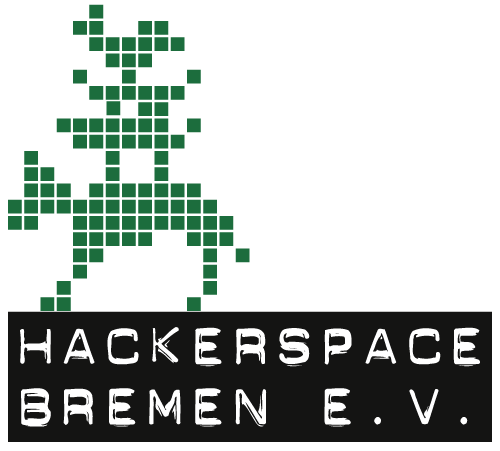
\includegraphics[width=1.1\textwidth]{HSpaceHBLogo}
\caption{Hackerspace Logo}
\label{fig:HSHBLogo}
\end{figure}

Dies ist ein Typoblindtext. An ihm kann man sehen, ob alle Buchstaben da sind und wie sie aussehen. Manchmal benutzt man Worte wie Hamburgefonts, Rafgenduks oder Handgloves, um Schriften zu testen. Manchmal Sätze, die alle Buchstaben des Alphabets enthalten - man nennt diese Sätze »Pangrams«. Sehr bekannt ist dieser: The quick brown fox jumps over the lazy old dog. Oft werden in Typoblindtexte auch fremdsprachige Satzteile eingebaut (AVAIL® and Wefox™ are testing aussi la Kerning), um die Wirkung in anderen Sprachen zu testen. In Lateinisch sieht zum Beispiel fast jede Schrift gut aus. Quod erat demonstrandum. Seit 1975 fehlen in den meisten Testtexten die Zahlen, weswegen nach TypoGb. 204 § ab dem Jahr 2034 Zahlen in 86 der Texte zur Pflicht werden. Nichteinhaltung wird mit bis zu 245 \euro{} oder 368 \$ bestraft. Genauso wichtig in sind mittlerweile auch Âçcèñtë, die in neueren Schriften aber fast immer enthalten sind. Ein wichtiges aber schwierig zu integrierendes Feld sind OpenType-Funktionalitäten. Je nach Software und Voreinstellungen können eingebaute Kapitälchen, Kerning oder Ligaturen (sehr pfiffig) nicht richtig dargestellt werden.
\begin{table}[htb]
	\caption{Eine Tabelle}
	\label{tab:tabelle1}
	\centering
	\begin{tabular}{ccc}
		a & b & c\\
		d & e & f
	\end{tabular}
\end{table}

Dies ist ein Typoblindtext. An ihm kann man sehen, ob alle Buchstaben da sind und wie sie aussehen. Manchmal benutzt man Worte wie Hamburgefonts, Rafgenduks oder Handgloves, um Schriften zu testen. Manchmal Sätze, die alle Buchstaben des Alphabets enthalten - man nennt diese Sätze »Pangrams«. Sehr bekannt ist dieser: The quick brown fox jumps over the lazy old dog. Oft werden in Typoblindtexte auch fremdsprachige Satzteile eingebaut (AVAIL® and Wefox™ are testing aussi la Kerning), um die Wirkung in anderen Sprachen zu testen. In Lateinisch sieht zum Beispiel fast jede Schrift gut aus. Quod erat demonstrandum. Seit 1975 fehlen in den meisten Testtexten die Zahlen, weswegen nach TypoGb. 204 § ab dem Jahr 2034 Zahlen in 86 der Texte zur Pflicht werden. Nichteinhaltung wird mit bis zu 245 \euro{} oder 368 \$ bestraft. Genauso wichtig in sind mittlerweile auch Âçcèñtë, die in neueren Schriften aber fast immer enthalten sind. Ein wichtiges aber schwierig zu integrierendes Feld sind OpenType-Funktionalitäten. Je nach Software und Voreinstellungen können eingebaute Kapitälchen, Kerning oder Ligaturen (sehr pfiffig) nicht richtig dargestellt werden.
\begin{table}[htb]
	\caption{Hässliche Tabelle}
	\label{tab:tabelle2}
	\centering
	\begin{tabular}{|c|c|c|}
		\hline
		a & b & c\\
		\hline
		d & e & f\\
		\hline
	\end{tabular}
\end{table}
\begin{table}[htb]
	\caption{Bessere Tabelle}
	\label{tab:tabelle3}
	\centering
	\begin{tabular}{ccc}
		\toprule
		a & b & c\\
		\midrule
		d & e & f\\
		g & h & i\\
		\bottomrule
	\end{tabular}
\end{table}


\end{document}